\begin{figure}[!htbp]
\begin{center}
\thinmuskip=-2mu
\thickmuskip=-2mu
\nulldelimiterspace=-1pt
\scriptspace=0pt
\begin{subfigure}[b]{0.80\columnwidth}
  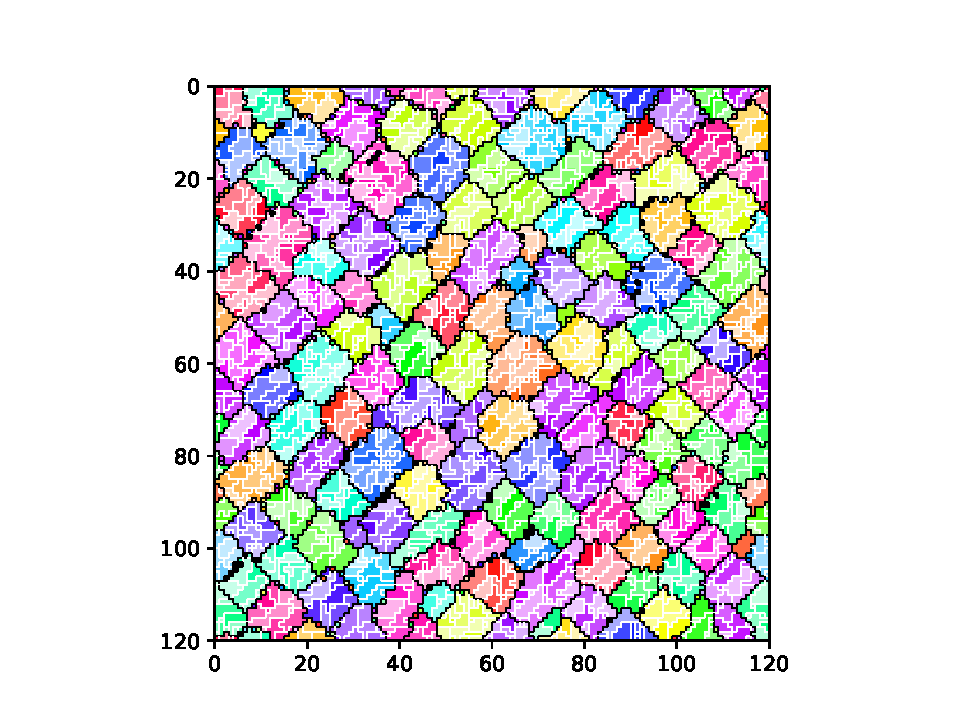
\includegraphics[width=\columnwidth,trim={2.5cm 0.5cm 2.5cm 1cm},clip]{img/ChannelMap_1022_update19500000}
  \caption{Mean $P_{c} = 0.77$, $P_0 = 0.09$, $P_1 = 0.14$; gen. 20,475}
  \label{fig:ChannelMap_1022}
\end{subfigure}

\begin{subfigure}[b]{0.80\columnwidth}
  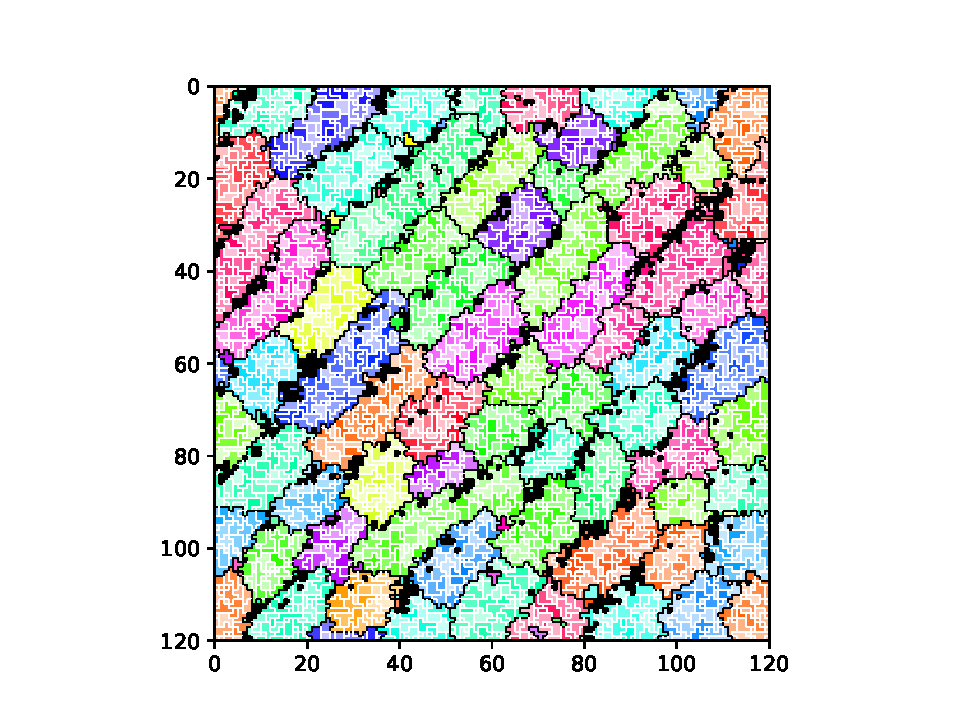
\includegraphics[width=\columnwidth,trim={2.5cm 0.5cm 2.5cm 1cm},clip]{img/ChannelMap_1041_update19500000}
  \caption{Mean $P_0 = 1.0$; gen. 23,971}
  \label{fig:ChannelMap_1041}
\end{subfigure}

\begin{subfigure}[b]{0.80\columnwidth}
  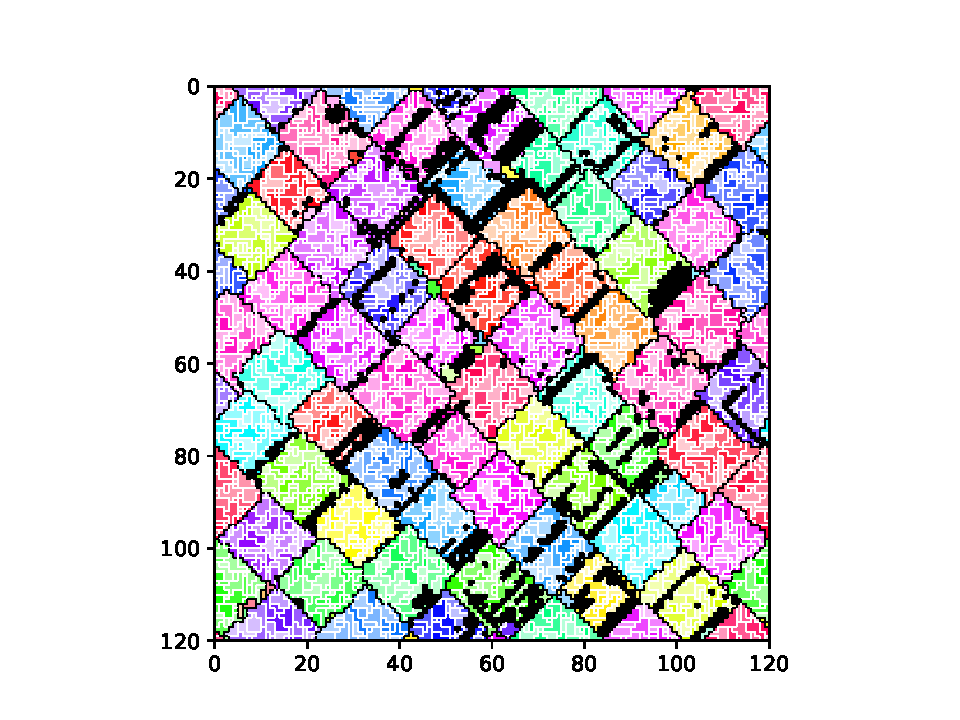
\includegraphics[width=\columnwidth,trim={2.5cm 0.5cm 2.5cm 1cm},clip]{img/ChannelMap_1008_update19500000}
  \caption{Mean $P_1 = 1.0$; gen. 25,841}
  \label{fig:ChannelMap_1008}
\end{subfigure}

\caption{
End state of same-channel signaling networks in replicates where cell- (\ref{fig:ChannelMap_1022}), zeroth- (\ref{fig:ChannelMap_1041}), and first-level (\ref{fig:ChannelMap_1008}) individuality dominated.
Level-zero channels are coded by color value and level-one channels are coded by hue.
}
\label{fig:outcome_grids}
\end{center}
\end{figure}
